\subsection{Bioacoustic Index}
The bioacoustic index was originally developed by ecologists studying the effects of invasive species on the native bird population of Hawaii. The purpose of such an index was to create a metric that closely correlated to the actual population of birds within an environment. This way, the researchers could have a reasonable estimation of the amount of birds within a given area without having to count them all by hand all the time.\par
This metric works by first specifying a range of frequencies (in Hz) at which biophony (or just about any type of sound that researchers expect to target) is expected to occur. Then, within this range of frequencies, measure the power (in Db) produced from these recordings within bins of specified ranges of time (in s). This should result in a collection of segments of curves of power. Finally, through determining the average area underneath these curves, the bioacoustic index value is found.\par
For the original researchers, this metric proved to be quite useful. By measuring the amount of birds at each of their research sites and comparing that amount to the respectively observed bioacoustic index, they were able to produce a regression model with an r-squared value of .97 (see Figure \ref{fig:BiCorrelation}), thus making future estimates of avian population easier to make automatically with just audio recordings.\cite{boelman}\par
Of course, however, this metric has some drawbacks. Namely, it requires knowledge of the environment that the field work is occurring in. In order for this metric to be used effectively, researchers need to know beforehand the frequency range they intend to target and the correlation factor between the actual population count and the bioacoustic index value. Both of these variables require preliminary study to obtain before the bioacoustic index can return meaningful data.\par
\begin{figure}
  \begin{center}
    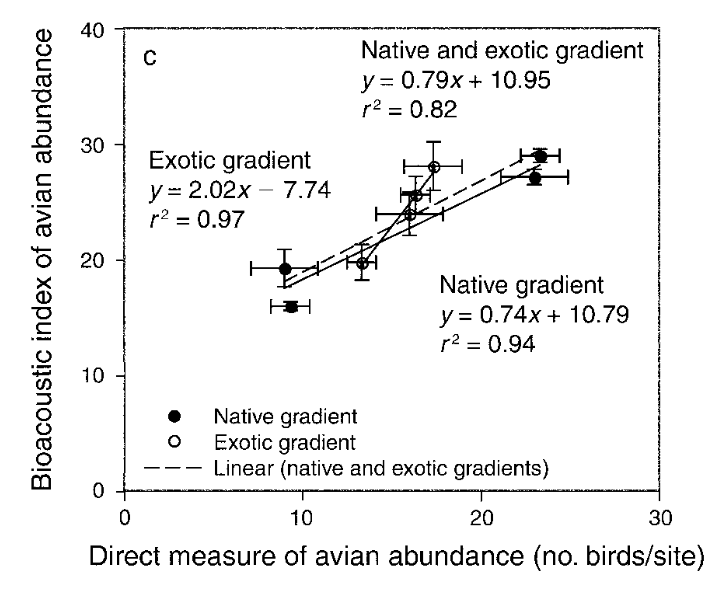
\includegraphics[width=0.7\textwidth]{BiCorrelation}
  \end{center}
  \caption{Relation between the measured amount of birds at a research site and the bioacoustic index observed at the site}
  \label{fig:BiCorrelation}
\end{figure}
